%&preformat-synopsis
\RequirePackage[l2tabu,orthodox]{nag} % Раскомментировав, можно в логе получать рекомендации относительно правильного использования пакетов и предупреждения об устаревших и нерекомендуемых пакетах

% Откомментируйте, чтобы отключить генерацию закладок в pdf
% \PassOptionsToPackage{bookmarks=false}{hyperref}
\documentclass[a4paper,14pt,twoside,openany,article]{memoir} %,draft

\input{common/setup}          % общие настройки шаблона
\input{common/packages}       % Пакеты общие для диссертации и автореферата
\synopsistrue                 % Этот документ --- автореферат
\input{Synopsis/synpackages}  % Пакеты для автореферата
\input{Synopsis/userpackages} % Пакеты для специфических пользовательских задач

\input{common/newnames}       % Новые переменные, которые могут использоваться во всём проекте
\input{Synopsis/setup}        % Упрощённые настройки шаблона

%%% Основные сведения новой диссертации %%%
% Содержательные данные взяты из канонических материалов ВЕРСИЯ_3.
% Поля, отсутствующие в этих материалах, отмечены как требующие уточнения.

\newcommand{\thesisAuthorLastName}{Корнеева}
\newcommand{\thesisAuthorOtherNames}{Анна Дмитриевна}
\newcommand{\thesisAuthorInitials}{А.\,Д.}
\newcommand{\thesisAuthor}{%
	\texorpdfstring{\thesisAuthorLastName~\thesisAuthorOtherNames}%
	{\thesisAuthorLastName, \thesisAuthorOtherNames}%
}
\newcommand{\thesisAuthorShort}{\thesisAuthorInitials~\thesisAuthorLastName}

% Рабочее название следует подтвердить по утверждённым документам соискателя.
\newcommand{\thesisTitle}%
{Правовая культура Каталонии XII--XIII~вв.: тексты, язык и~судебное доказательство}
\newcommand{\thesisSpecialtyNumber}{5.6.2}
\newcommand{\thesisSpecialtyTitle}{Всеобщая история}
\newcommand{\thesisDegree}{кандидата исторических наук}
\newcommand{\thesisDegreeShort}{канд. ист. наук}
\newcommand{\thesisCity}{Москва}
\newcommand{\thesisYear}{2026}

\newcommand{\thesisOrganization}{\textit{сведения уточняются}}
\newcommand{\thesisOrganizationShort}{\textit{сведения уточняются}}
\newcommand{\thesisInOrganization}{\textit{сведения уточняются}}

\newcommand{\supervisorFio}{\textit{сведения уточняются}}
\newcommand{\supervisorRegalia}{\textit{сведения уточняются}}
\newcommand{\supervisorFioShort}{\textit{сведения уточняются}}
\newcommand{\supervisorRegaliaShort}{\textit{сведения уточняются}}

% Эти поля требуются автореферату, но не используются в основном тексте диссертации.
\newcommand{\opponentOneFio}{\textit{сведения уточняются}}
\newcommand{\opponentOneRegalia}{\textit{сведения уточняются}}
\newcommand{\opponentOneJobPlace}{\textit{сведения уточняются}}
\newcommand{\opponentOneJobPost}{\textit{сведения уточняются}}
\newcommand{\opponentTwoFio}{\textit{сведения уточняются}}
\newcommand{\opponentTwoRegalia}{\textit{сведения уточняются}}
\newcommand{\opponentTwoJobPlace}{\textit{сведения уточняются}}
\newcommand{\opponentTwoJobPost}{\textit{сведения уточняются}}
\newcommand{\leadingOrganizationTitle}{\textit{сведения уточняются}}
\newcommand{\defenseDate}{\textit{сведения уточняются}}
\newcommand{\defenseCouncilNumber}{\textit{сведения уточняются}}
\newcommand{\defenseCouncilTitle}{\textit{сведения уточняются}}
\newcommand{\defenseCouncilAddress}{\textit{сведения уточняются}}
\newcommand{\defenseCouncilPhone}{\textit{сведения уточняются}}
\newcommand{\defenseSecretaryFio}{\textit{сведения уточняются}}
\newcommand{\defenseSecretaryRegalia}{\textit{сведения уточняются}}
\newcommand{\synopsisLibrary}{\textit{сведения уточняются}}
\newcommand{\synopsisDate}{\textit{сведения уточняются}}

\providecommand{\keywords}%
{Каталония, Средние века, обычное право, правовая культура, историческая текстология,
старокаталанский язык, латынь, судебное доказательство, цифровые методы}
           % Основные сведения
% Данные автореферата по замечаниям учёного секретаря к версии v4.
% Переопределения локальны для сборки synopsis; common/data.tex не меняется.
\renewcommand{\opponentOneRegalia}{доктор технических наук, член-корреспондент РАН}
\renewcommand{\opponentOneJobPlace}{Научно-исследовательский институт прикладной механики и~электродинамики МАИ}
\renewcommand{\opponentOneJobPost}{директор}
\renewcommand{\opponentTwoJobPlace}{Институт космических исследований РАН}
\renewcommand{\opponentTwoJobPost}{научный сотрудник}
\renewcommand{\defenseDate}{1 декабря 2026~года}
\renewcommand{\defenseSecretaryRegalia}{канд. физ.-мат. наук, доцент}
\renewcommand{\synopsisDate}{«\blank[1cm]» \blank[3.5cm] 2026~г.}
\setcounter{showmailingdate}{1}
       % Сведения только для автореферата
%%% Кодировки и шрифты %%%
\ifxetexorluatex
    % Язык по-умолчанию русский с поддержкой приятных команд пакета babel
    \setmainlanguage[babelshorthands=true]{russian}
    % Языки библиографии: langid выбирает локальные сокращения и переносы.
    \setotherlanguages{english,catalan,french,german,italian,latin,portuguese,spanish}

    % Проверка существования шрифтов. Недоступна в pdflatex
    \ifnumequal{\value{fontfamily}}{1}{
        \IfFontExistsTF{Times New Roman}{}{\setcounter{fontfamily}{0}}
    }{}
    \ifnumequal{\value{fontfamily}}{2}{
        \IfFontExistsTF{LiberationSerif}{}{\setcounter{fontfamily}{0}}
    }{}

    \ifnumequal{\value{fontfamily}}{0}{% Семейство шрифтов CMU. Используется как fallback
        \setmonofont[
          BoldFont={cmuntb.otf},
          ItalicFont={cmunit.otf},
          BoldItalicFont={cmuntx.otf}
        ]{cmuntt.otf} % {CMU Typewriter Text} % моноширинный шрифт
        \newfontfamily\cyrillicfonttt[
          BoldFont={cmuntb.otf},
          ItalicFont={cmunit.otf},
          BoldItalicFont={cmuntx.otf}
        ]{cmuntt.otf} % {CMU Typewriter Text} % моноширинный шрифт для кириллицы
        \defaultfontfeatures{Ligatures=TeX}   % стандартные лигатуры TeX, замены нескольких дефисов на тире и т. п. Настройки моноширинного шрифта должны идти до этой строки, чтобы при врезках кода программ в коде не применялись лигатуры и замены дефисов
        \setmainfont[
          SlantedFont={cmunsl.otf},
          BoldSlantedFont={cmunbl.otf},
          BoldFont={cmunbx.otf},
          ItalicFont={cmunti.otf},
          BoldItalicFont={cmunbi.otf}
        ]{cmunrm.otf} % {CMU Serif}           % Шрифт с засечками
        \newfontfamily\cyrillicfont[
          SlantedFont={cmunsl.otf},
          BoldSlantedFont={cmunbl.otf},
          BoldFont={cmunbx.otf},
          ItalicFont={cmunti.otf},
          BoldItalicFont={cmunbi.otf}
        ]{cmunrm.otf}   % {CMU Serif}         % Шрифт с засечками для кириллицы
        \setsansfont[
          BoldFont={cmunsx.otf},
          ItalicFont={cmunsi.otf},
          BoldItalicFont={cmunso.otf}
        ]{cmunss.otf} % {CMU Sans Serif}      % Шрифт без засечек
        \newfontfamily\cyrillicfontsf[
          BoldFont={cmunsx.otf},
          ItalicFont={cmunsi.otf},
          BoldItalicFont={cmunso.otf}
        ]{cmunss.otf} % {CMU Sans Serif}      % Шрифт без засечек для кириллицы
    }

    \ifnumequal{\value{fontfamily}}{1}{                    % Семейство MS шрифтов
        \setmonofont{Times New Roman}                      % единый шрифт, включая листинги
        \newfontfamily\cyrillicfonttt{Times New Roman}     % единый шрифт для кириллицы
        \defaultfontfeatures{Ligatures=TeX}                % стандартные лигатуры TeX, замены нескольких дефисов на тире и т. п. Настройки моноширинного шрифта должны идти до этой строки, чтобы при врезках кода программ в коде не применялись лигатуры и замены дефисов
        \setmainfont{Times New Roman}                      % Шрифт с засечками
        \newfontfamily\cyrillicfont{Times New Roman}       % Шрифт с засечками для кириллицы
        \setsansfont{Times New Roman}                      % единый шрифт во всём документе
        \newfontfamily\cyrillicfontsf{Times New Roman}     % единый шрифт для кириллицы
        \ifxetex
            \setmathsfont(Digits,Latin,Greek){Times New Roman}
            \setmathrm{Times New Roman}
            \setmathsf{Times New Roman}
            \setmathtt{Times New Roman}
        \fi
    }

    \ifnumequal{\value{fontfamily}}{2}{                    % Семейство шрифтов Liberation (https://pagure.io/liberation-fonts)
        \setmonofont{LiberationMono}[Scale=0.87] % моноширинный шрифт
        \newfontfamily\cyrillicfonttt{LiberationMono}[     % моноширинный шрифт для кириллицы
            Scale=0.87]
        \defaultfontfeatures{Ligatures=TeX}                % стандартные лигатуры TeX, замены нескольких дефисов на тире и т. п. Настройки моноширинного шрифта должны идти до этой строки, чтобы при врезках кода программ в коде не применялись лигатуры и замены дефисов
        \setmainfont{LiberationSerif}                      % Шрифт с засечками
        \newfontfamily\cyrillicfont{LiberationSerif}       % Шрифт с засечками для кириллицы
        \setsansfont{LiberationSans}                       % Шрифт без засечек
        \newfontfamily\cyrillicfontsf{LiberationSans}      % Шрифт без засечек для кириллицы
    }

\else
    \ifnumequal{\value{usealtfont}}{1}{% Используется pscyr, при наличии
        \IfFileExists{pscyr.sty}{\renewcommand{\rmdefault}{ftm}}{}
    }{}
\fi
          % Определение шрифтов (частичное)
\input{common/styles}         % Стили общие для диссертации и автореферата
%%% Изображения %%%
\graphicspath{{images/}{Synopsis/images/}}         % Пути к изображениям

%%% Макет страницы %%%
\geometry{a4paper, top=30mm, bottom=20mm, left=20mm, right=20mm, headheight=17pt, headsep=8mm, nomarginpar}%, showframe
\setlength{\topskip}{14pt}   %размер дополнительного верхнего поля

%%% Интервалы %%%
%% Реализация средствами класса (на основе setspace) ближе к типографской классике.
%% И правит сразу и в таблицах (если со звёздочкой)
%\DoubleSpacing*     % Двойной интервал
%\OnehalfSpacing*    % Полуторный интервал
\SingleSpacing      % Одинарный интервал
%\setSpacing{1.42}   % Полуторный интервал, подобный Ворду (возможно, стоит включать вместе с предыдущей строкой)

%%% Выравнивание и переносы %%%
%% http://tex.stackexchange.com/questions/241343/what-is-the-meaning-of-fussy-sloppy-emergencystretch-tolerance-hbadness
%% http://www.latex-community.org/forum/viewtopic.php?p=70342#p70342
\tolerance 1414
\hbadness 1414
\emergencystretch 1.5em % В случае проблем регулировать в первую очередь
\hfuzz 0.3pt
\vfuzz \hfuzz
%\raggedbottom
%\sloppy                 % Избавляемся от переполнений
\clubpenalty=10000      % Запрещаем разрыв страницы после первой строки абзаца
\widowpenalty=10000     % Запрещаем разрыв страницы после последней строки абзаца

%%% Колонтитулы %%%
\makeevenhead{plain}{}{\thepage}{}
\makeoddhead{plain}{}{\thepage}{}
\makeevenfoot{plain}{}{}{}
\makeoddfoot{plain}{}{}{}
\pagestyle{plain}

%%% Размеры заголовков %%%
\setsecheadstyle{\normalfont\large\bfseries}
\renewcommand*{\chaptitlefont}{\normalfont\large\bfseries}

%%% Подписи %%%
\setfloatadjustment{table}{%
    \setlength{\abovecaptionskip}{0pt}   % Отбивка над подписью
    \setlength{\belowcaptionskip}{0pt}   % Отбивка под подписью
}

%%% Отступы у плавающих блоков %%%
\setlength\textfloatsep{1ex}
\setlength\intextsep{1ex}

%%% Компактная вёрстка списков и выключных формул %%%
\setlist[enumerate]{nosep,labelindent=0pt,leftmargin=1.8em,labelsep=0.5em,beginpenalty=10000}
\setlength{\abovedisplayskip}{4pt plus 1pt minus 1pt}
\setlength{\belowdisplayskip}{4pt plus 1pt minus 1pt}
\setlength{\abovedisplayshortskip}{2pt plus 1pt minus 1pt}
\setlength{\belowdisplayshortskip}{3pt plus 1pt minus 1pt}

% Макет А4 для уменьшения при печати брошюры: основной текст 14 pt.
\makeatletter
\renewcommand{\normalsize}{\@setfontsize\normalsize{14pt}{16pt}%
    \abovedisplayskip=6pt plus 1pt minus 1pt
    \belowdisplayskip=6pt plus 1pt minus 1pt
    \abovedisplayshortskip=3pt plus 1pt minus 1pt
    \belowdisplayshortskip=4pt plus 1pt minus 1pt}
\makeatother
\AtBeginDocument{\normalsize\setlength{\parindent}{1cm}\setlength{\parskip}{0pt}}
\setsecheadstyle{\centering\normalfont\bfseries\large}
\setbeforesecskip{8pt}
\setaftersecskip{8pt}
\DeclareCaptionLabelSeparator{synopsisemdash}{~---~}
\captionsetup[figure]{font=normalsize,labelsep=synopsisemdash,skip=4pt}
\captionsetup[table]{font=normalsize,labelsep=synopsisemdash,skip=4pt}
\setlength{\intextsep}{8pt}
\setlength{\textfloatsep}{10pt}
\urlstyle{same}
    % Стили для автореферата
\input{Synopsis/userstyles}   % Стили для специфических пользовательских задач

%%% Библиография. Выбор движка для реализации %%%
\ifnumequal{\value{bibliosel}}{0}{%
    \input{biblio/predefined} % Встроенная реализация с загрузкой файла через движок bibtex8
}{
    \input{biblio/biblatex}   % Реализация пакетом biblatex через движок biber
}

% В работах о платформах перечисляем авторов до соискателя включительно.
\AtEveryBibitem{%
    \ifboolexpr{test {\iffieldequalstr{entrykey}{korneev_mars_platform_2024}}
        or test {\iffieldequalstr{entrykey}{korneev_venus_platform_2026}}}
        {\defcounter{maxnames}{2}\defcounter{minnames}{2}}{}%
}

% Вывести информацию о выбранных опциях в лог сборки
\typeout{Selected options:}
\typeout{Draft mode: \arabic{draft}}
\typeout{Font: \arabic{fontfamily}}
\typeout{AltFont: \arabic{usealtfont}}
\typeout{Bibliography backend: \arabic{bibliosel}}
\typeout{Precompile images: \arabic{imgprecompile}}
% Вывести информацию о версиях используемых библиотек в лог сборки
\listfiles

\begin{document}
%%% Переопределение именований типовых разделов
% https://tex.stackexchange.com/a/156050
\gappto\captionsrussian{\input{common/renames}} % for polyglossia and babel
\input{common/renames}

\thispagestyle{empty}
\begingroup
\setlength{\parindent}{0pt}
\begin{flushright}
\textit{На правах рукописи}
\end{flushright}
\vspace*{42mm}
\begin{center}
{\normalfont\normalsize \thesisAuthor\par}
\vspace{18mm}
{\bfseries\normalsize\MakeUppercase{\thesisTitle}\par}
\vspace{22mm}
Специальность \thesisSpecialtyNumber~--- \thesisSpecialtyTitle
\vspace{20mm}

Автореферат диссертации на соискание учёной степени\par
\thesisDegree
\end{center}
\vfill
{\centering\thesisCity~--- \thesisYear\par}
\endgroup

\newpage
\thispagestyle{empty}
\begingroup
\setlength{\parindent}{0pt}
\setlength{\parskip}{0pt}
\noindent Работа выполнена в~\thesisInOrganization.

\vspace{6mm}
\textbf{Научный руководитель:}\par\nobreak\vspace{2mm}
\textbf{\supervisorFio}, \supervisorRegalia\space
ИПМ им.~М.\,В.~Келдыша РАН.

\vspace{6mm}
\textbf{Официальные оппоненты:}\par\nobreak\vspace{2mm}
\textbf{\opponentOneFio}, \opponentOneRegalia,
\opponentOneJobPost\space\synopsisOpponentOneJobPlaceGenitive.

\vspace{4mm}
\textbf{\opponentTwoFio}, \opponentTwoRegalia,
\opponentTwoJobPost\space\synopsisOpponentTwoJobPlaceGenitive.

\vspace{6mm}
\textbf{Ведущая организация:}\par\nobreak\vspace{2mm}
\leadingOrganizationTitle.

\vspace{8mm}
Защита состоится \defenseDate~в~\synopsisDefenseTime~на~заседании диссертационного совета \defenseCouncilNumber, созданного на~базе \defenseCouncilTitle, по~адресу: \defenseCouncilAddress.

\vspace{6mm plus1fill}
\hyphenation{сайте}
С~диссертацией можно ознакомиться в~библиотеке и~на~сайте\par\nobreak
\mbox{ИПМ им.~М.\,В.~Келдыша РАН} \url{https://keldysh.ru/council/1/}

\vspace{16mm plus1fill}
Автореферат разослан \synopsisDate

\vfill
\begin{tabularx}{\textwidth}{@{}Xr@{}}
Учёный секретарь & \\
диссертационного совета \defenseCouncilNumber & \\
\defenseSecretaryRegalia & \defenseSecretaryFio
\end{tabularx}
\endgroup
        % Титульный лист
%\mainmatter                   % В том числе начинает нумерацию страниц арабскими цифрами с единицы
\mainmatter*                  % Нумерация страниц не изменится, но начнётся с новой страницы
\raggedbottom                 % Не растягивать вертикальные отбивки на неполных страницах
\pdfbookmark{Общая характеристика работы}{characteristic}
\section*{Общая характеристика работы}

\newcommand{\synopsisheading}[2]{%
    \pdfbookmark[1]{#1}{#2}%
    \par\addvspace{3pt}\noindent\textbf{#1.}\enspace%
}

\synopsisheading{Актуальность темы исследования}{actuality}
Электрореактивные двигательные установки (ЭРДУ) расширяют множество доступных баллистических схем межпланетных миссий, особенно для малых космических аппаратов (КА): высокий удельный импульс позволяет получить большой располагаемый запас характеристической скорости при ограниченной массе рабочего тела. Однако малая тяга требует длительного управляемого движения, а~характеристики перелёта существенно зависят от~даты старта, продолжительности перелёта, целевой орбиты, параметров КА и~двигателя.

На~ранних этапах баллистического проектирования требуются массовые расчёты траекторий при различных наборах параметров. Численное решение каждой задачи оптимального управления вычислительно затратно. Конечные формулы и~асимптотические решения сокращают затраты лишь для близких орбит, усреднённых многовитковых перелётов и~других упрощённых постановок. Для межпланетных перелётов с~малым числом витков, существенным изменением радиуса орбиты и~непериодическим управлением универсальные компактные формулы не~получены.

Номограммы связывают дату старта, продолжительность перелёта и~его энергетические характеристики и~служат для предварительного выбора траектории. При непрерывной тяге изолинии могут расслаиваться на~области с~разным числом витков. Поэтому выбор окна старта неотделим от~выбора семейства траекторий. Непрямое уточнение требует согласованных с~этим семейством начальных значений сопряжённых переменных: произвольное приближение может привести к~другому локальному решению или отсутствию сходимости.

Актуально построение промежуточного численно-аналитического представления, связывающего результаты массового расчёта энергетически оптимальных траекторий с~компактными конечными формулами. Оно должно быть интерпретируемым, сохранять структуру оптимальных решений и~начальные значения сопряжённых переменных, обеспечивать выбор семейства траекторий и~быстрое построение начального приближения. Таким представлением служит модельное многообразие решений задачи встречи.

\synopsisheading{Степень разработанности темы исследования}{elaboration}
С~работами школы Д.Е.~Охоцимского связана отечественная традиция постановки и~численного исследования задач космической динамики. Т.М.~Энеевым и~соавторами развивались методы проектирования траекторий с~малой тягой и~графические средства предварительного баллистического анализа.

Теоретической основой непрямой оптимизации служит принцип максимума Л.С.~Понтрягина. В.Г.~Петуховым развиты методы оптимизации многовитковых перелётов и~продолжения по~параметрам граничных условий. М.С.~Константиновым исследованы прикладные задачи оптимизации гелиоцентрических траекторий с~ЭРДУ. Близкое направление, основанное на~дискретных псевдоимпульсах, систематизировано Ю.П.~Улыбышевым.

Конечные зависимости для ряда квазикруговых, эллиптических и~неэкваториальных постановок с~малой тягой получены С.~да~Силва Фернандесом и~его соавторами. Методы усреднения и~аналитические приближения развивались С.~Жеффруа и~Р.~Эпенуа, А.~Петропулосом и~Р.П.~Расселлом; отдельные специальные режимы исследованы Ж.А.~Кечичяном и~Д.М.~Азимовым.

Современные численные подходы включают прямые, непрямые, гибридные и~эвристические методы. Гомотопический переход от~упрощённой постановки к~задаче минимального расхода исследован Т.~Хаберкорном и~Ж.~Жерго, а~также Ф.~Цзяном и~его соавторами. Б.~Паном и~соавторами предложены двойная и~вероятностная гомотопии; дальнейшее исследование пространства решений и~варианты продолжения представлены в~работах Ц.~Чжана и~Я.~Вана. Эти методы позволяют прослеживать ветви решений, но~не~устраняют неединственность решения краевой задачи и~её чувствительность к~начальному приближению.

Возможность символьного восстановления физических закономерностей показана М.~Шмидтом и~его соавторами; физически ориентированный алгоритм предложен С.-М.~Удреску, а~практический инструментарий PySR развит М.~Крэнмером.

Символьная регрессия применяется к~структурированному множеству решений с~регулярной параметризацией после анализа структуры модельного многообразия и~нормировки переменных.

\synopsisheading{Цель работы}{aim}
Цель работы --- разработка и~апробация численно-аналитического метода построения начального приближения, согласованного с~выбранным семейством траекторий в~расслоении по~числу витков, для энергетически оптимальных межпланетных перелётов с~идеально регулируемой тягой на~основе модельного многообразия решений задачи встречи.

Для достижения цели поставлены \textbf{задачи}:
\begin{enumerate}[beginpenalty=10000]
    \item разработать методику построения и~аппроксимации модельного многообразия решений задачи встречи с~идеально регулируемой тягой для исследования расслоения по~числу витков;
    \item исследовать многообразие решений в~плоской круговой модели, выделить точки оптимальной дальности и~построить конечные формулы, связывающие параметры компланарного перелёта между круговыми орбитами с~характеристиками траектории и~начальными значениями сопряжённых переменных;
    \item разработать линейные преобразования начальных значений сопряжённых переменных для учёта изменения начального фазового вектора, эллиптичности и~пространственной ориентации конечной орбиты при переходе от~плоской круговой модели к~целевой задаче встречи;
    \item построить и~апробировать алгоритм формирования по~дате старта и~параметрам задачи встречи начального приближения для выбранного семейства траекторий; проверить его на~перелётах Земля--Марс и~Земля--Венера, в~постановках с~начальным дополнительным импульсом скорости и~при продолжении к~постановке с~постоянной скоростью истечения.
\end{enumerate}

\synopsisheading{Объект и предмет исследования}{objectsubject}
Объект исследования --- семейства энергетически оптимальных решений задач встречи для межпланетных перелётов космического аппарата с~идеально регулируемой непрерывной тягой, рассматриваемые с~точки зрения расслоения по~числу витков. Предмет исследования --- численно-аналитические методы построения, исследования, аппроксимации и~использования модельного многообразия решений задачи встречи с~идеально регулируемой тягой, позволяющие описывать расслоение по~числу витков и~формировать начальное приближение, согласованное с~выбранным семейством траекторий.

\synopsisheading{Положения, выносимые на защиту}{defpositions}
На~защиту выносятся:
\begin{enumerate}[beginpenalty=10000]
    \item предложена методика исследования расслоения решений задачи встречи с~идеально регулируемой тягой по~числу витков. Модельное многообразие решений двухточечной краевой задачи строится дискретным продолжением по~параметрической сетке, а~его характеристики аппроксимируются. Точки оптимальной дальности служат основным объектом аппроксимации и~выбора начального приближения;

    \item для плоской круговой модели предложены построенные методом символьной регрессии конечные формулы, позволяющие по~параметрам компланарного перелёта между круговыми орбитами выбирать точку оптимальной дальности и~вычислять продолжительность перелёта, квадратичный функционал, начальную синодическую фазу и~начальные значения сопряжённых переменных ИРТ-траектории;

    \item разработан аппарат линейных преобразований начальных значений сопряжённых переменных для перехода от~плоской круговой модели к~целевой задаче встречи с~учётом изменения начального фазового вектора, эллиптичности и~пространственной ориентации конечной орбиты. Предложены конечные формулы для управляющих параметров преобразований и~линейная коррекция витковой дальности;

    \item построен и~апробирован алгоритм формирования начального приближения, согласованного с~семейством траекторий в~расслоении по~числу витков. По~дате старта и~параметрам целевой задачи он формирует параметры модельной постановки, выбирает точку оптимальной дальности, вычисляет продолжительность перелёта и~линейными преобразованиями переносит начальные значения сопряжённых переменных к~целевой задаче. На~перелётах Земля--Марс и~Земля--Венера показано успешное численное уточнение траекторий, в~том числе при дополнительном импульсе скорости в~начальный момент времени и~продолжении к~постановке с~постоянной скоростью истечения.
\end{enumerate}

\synopsisheading{Научная новизна}{novelty}
Научная новизна работы состоит в~следующем:
\begin{enumerate}[beginpenalty=10000]
    \item разработана методика применения символьной регрессии для построения интерпретируемых конечных формул, аппроксимирующих характеристики решений задачи встречи с~идеально регулируемой тягой и~пригодных для формирования начальных приближений;
    \item предложен подход к~описанию расслоения решений задачи встречи с~идеально регулируемой тягой, в~котором структура расслоения задаётся пересечениями изолиний начальной синодической фазы с~кривой локальных оптимумов в~точках оптимальной дальности;
    \item на~основе инвариантов, связанных с~первыми интегралами расширенной системы уравнений движения, получены условия на~допустимый вид линейных преобразований начальных значений сопряжённых переменных;
    \item разработан алгоритм построения начального приближения, основанный на~согласованном выборе семейства траекторий, продолжительности перелёта и~начальных значений сопряжённых переменных.
\end{enumerate}

\synopsisheading{Теоретическая и практическая значимость}{significance}
Теоретическая значимость работы состоит в~исследовании структуры модельного многообразия энергетически оптимальных решений задачи встречи и~построении конечных формул, связывающих параметры модельной постановки с~характеристиками оптимальной траектории и~начальными значениями сопряжённых переменных. Предложенные линейные преобразования задают численно-аналитический способ перехода от~плоской круговой модели к~более общим пространственным и~эллиптическим постановкам.

Практическая значимость состоит в~возможности использовать предложенные формулы для быстрого построения начальных приближений при проектно-баллистическом анализе межпланетных миссий с~ЭРДУ. Это позволяет сократить число расчётов, выполняемых с~нуля, и~использовать аппроксимированное модельное многообразие как промежуточное численно-аналитическое представление между предварительным анализом миссии и~последующим численным уточнением траектории. Результаты реализованы в~\texttt{ILTT Toolbox}, апробированы на~перелётах Земля--Марс и~Земля--Венера и~использованы в~проектах РНФ №~19-11-00256 и~№~24-11-00038.

\synopsisheading{Методология и методы исследования}{methods}
В~работе используются методы теоретической механики, оптимального управления, небесной механики и~вычислительной математики. Математическая постановка основана на~уравнениях движения космического аппарата в~центральном гравитационном поле. Для сведения задачи оптимального управления к~двухточечной краевой задаче для фазовых и~сопряжённых переменных применяется принцип максимума Л.С.~Понтрягина. Основу методологии составляет построение регулярных связных ветвей решений энергетически оптимальных задач встречи, рассматриваемых как модельные многообразия. Для их численного построения используется дискретное продолжение по~параметрам граничных условий. Для зависимостей малой размерности с~регулярной структурой строится непосредственная аппроксимация. В~более сложных случаях применяется иерархический подход: выделяются более простые зависимости, а~возникающие коэффициент-функции аппроксимируются отдельно. Конечные формулы строятся методом символьной регрессии.\par\Needspace*{3\baselineskip}\noindent При их построении учитываются точность, корректность поведения на~рабочей области параметров, согласованность со~специальными случаями и~пригодность для дальнейшего использования. Для перехода к~пространственным и~эллиптическим постановкам используются линейные преобразования начальных значений сопряжённых переменных. Применимость подхода проверяется численным решением краевых задач и~массовыми вычислительными экспериментами на~наборах дат старта.

\synopsisheading{Степень достоверности результатов}{reliability}
Достоверность результатов обеспечивается согласованностью постановки с~необходимыми условиями оптимальности, контролем невязок двухточечной краевой задачи и~устойчивости перехода между соседними точками параметрической сетки. Конечные формулы проверены во~всей рассматриваемой области параметров, в~том числе при существенном изменении решений. Для линейных преобразований контролировались достижение целевых орбитальных элементов и~изменения витковой дальности и~большой полуоси конечной орбиты. Практическая проверка метода выполнена на~задачах перелёта Земля--Марс и~Земля--Венера. Оценены ошибки начального приближения, качество последующего уточнения и~вычислительные затраты по~сравнению с~альтернативными способами построения начального решения.

\synopsisheading{Апробация результатов работы}{probation}
Основные результаты диссертационной работы докладывались и~обсуждались на~следующих всероссийских и~международных научных конференциях:

\begin{enumerate}
    \item 12-й симпозиум Международной академии астронавтики по~будущему освоению космоса «Future Space Exploration»
    (Турин, Италия, 9--11 июня 2025~г.);

    \item Молодёжная научная конференция «Новые горизонты прикладной математики»
    (Москва, ИПМ им.~М.В.~Келдыша РАН, 17--18 апреля 2025~г.);

    \item 67-я Всероссийская научная конференция МФТИ
    (Москва, 31 марта -- 5 апреля 2025~г.);

    \item XLIX Академические чтения по~космонавтике, посвящённые памяти академика С.П.~Королёва и~других выдающихся отечественных учёных --- пионеров освоения космического пространства
    (Москва, МГТУ им.~Н.Э.~Баумана, 28--31 января 2025~г.);

    \item 23-я Международная конференция «Авиация и~космонавтика»
    (Москва, 18--22 ноября 2024~г.);

    \item XXIII Научно-техническая конференция молодых учёных и~специалистов ПАО «РКК „Энергия“ имени С.П.~Королёва»
    (Королёв, 28 октября -- 1 ноября 2024~г.);

    \item 75-й Международный астронавтический конгресс
    (Милан, Италия, 14--18 октября 2024~г.);

    \item Молодёжная научная конференция «Новые горизонты прикладной математики»
    (Москва, ИПМ им.~М.В.~Келдыша РАН, 18--19 апреля 2024~г.);

    \item XLVIII Академические чтения по~космонавтике
    (Москва, МГТУ им.~Н.Э.~Баумана, 23--26 января 2024~г.);

    \item 65-я Всероссийская научная конференция МФТИ
    (Москва, Долгопрудный, Жуковский, 3--8 апреля 2023~г.);

    \item XLVI Академические чтения по~космонавтике
    (Москва, МГТУ им.~Н.Э.~Баумана, 25--28 января 2022~г.);

    \item 64-я Всероссийская научная конференция МФТИ
    (Москва, Долгопрудный, Жуковский, 29 ноября -- 3 декабря 2021~г.);

    \item 63-я Всероссийская научная конференция МФТИ
    (Москва, Долгопрудный, Жуковский, 23--29 ноября 2020~г.).
\end{enumerate}

Результаты работы также обсуждались на~следующих научных семинарах:

\begin{enumerate}
    \item семинар «Динамика космических систем» отдела №~7 ИПМ им.~М.В.~Келдыша РАН
    (под руководством М.Ю.~Овчинникова);

    \item семинар по~механике, управлению и~информатике Института космических исследований РАН
    (под руководством Р.Р.~Назирова и~Н.А.~Эйсмонта);

    \item семинар по~теории управления и~динамике систем Института проблем механики им.~А.Ю.~Ишлинского РАН
    (под руководством академика Ф.Л.~Черноусько);

    \item семинар Баллистического центра ИПМ им.~М.В.~Келдыша РАН
    (под руководством А.Г.~Тучина);

    \item семинар «Механика и~управление движением» отдела №~5 ИПМ им.~М.В.~Келдыша РАН
    (под руководством Ю.Ф.~Голубева);

    \item семинар «Динамические системы и~механика» Московского авиационного института
    (под руководством Б.С.~Бардина и~П.С.~Красильникова);

    \item семинар «Механика космического полёта», проводимый на~кафедре «Космические системы и~ракетостроение» МАИ
    (под руководством члена-корреспондента РАН В.Г.~Петухова).
\end{enumerate}

\synopsisheading{Публикации}{publications}
По~теме диссертации имеется 6 публикаций в~журналах из~перечня ВАК, из~них 2 статьи индексируются в~Scopus и~Web of~Science. Всего опубликовано 19 научных работ, включая 13 работ в~изданиях и~материалах конференций, индексируемых в~РИНЦ. Получено свидетельство о~государственной регистрации программы для ЭВМ.


\synopsisheading{Личный вклад автора}{contribution}
Содержание диссертации и~основные положения, выносимые на~защиту, отражают персональный вклад автора в~опубликованные работы. Основные результаты, выносимые на~защиту, получены автором лично. Автором выполнены разработка расчётной схемы, построение и~исследование модельного многообразия, получение аппроксимационных формул, разработка линейных преобразований начальных значений сопряжённых переменных, программная реализация предложенного подхода и~проведение численных экспериментов. В~диссертации использованы результаты научных работ, выполненных автором лично и~в~соавторстве. В~совместных работах автору принадлежат результаты, составляющие основное содержание диссертации и~выносимые на~защиту.

\Needspace*{8\baselineskip}
\synopsisheading{Соответствие диссертации паспорту специальности}{specialty}
Диссертация соответствует научной специальности 1.1.7 «Теоретическая механика, динамика машин»: необходимые условия оптимальности и~сопряжённые переменные относятся к~аналитической динамике (направление~1), задача встречи --- к~управлению движением (направление~5), межпланетные перелёты --- к~астродинамике и~динамике летательных аппаратов (направления~9 и~10), построение модельного многообразия и~его аппроксимация --- к~математическому и~компьютерному моделированию (направление~14).

\synopsisheading{Объём и структура диссертации}{structure}
Диссертация состоит из~введения, четырёх глав, заключения и~трёх приложений. Полный объём составляет 198~страниц, включая 53~рисунка и~32~таблицы. Список литературы содержит 124~наименования.

\pdfbookmark[1]{Основное содержание работы}{main-content}
\section*{Основное содержание работы}

\noindent\textbf{В первой главе} разработана методика построения и~аппроксимации регулярной параметризованной ветви энергетически оптимальных решений задачи встречи. В~безразмерных переменных движение космического аппарата в~центральном гравитационном поле описывается системой
\begin{equation}
    \dot{\mathbf r}=\mathbf v,
    \qquad
    \dot{\mathbf v}=-\frac{\mathbf r}{r^3}+\mathbf a,
    \label{eq:syn-motion}
\end{equation}
а~критерием оптимальности служит квадратичный функционал
\begin{equation}
    J=\frac12\int_{t_0}^{t_f}\lVert\mathbf a(t)\rVert^2\,dt\longrightarrow\min.
    \label{eq:syn-functional}
\end{equation}
Здесь $\mathbf r$, $\mathbf v$ и~$\mathbf a$ --- безразмерные векторы положения, скорости и~реактивного ускорения, $r=\lVert\mathbf r\rVert$, а~$t_0$ и~$t_f$ --- начальный и~конечный моменты времени. Время перелёта $T=t_f-t_0$ и~состояния на~обоих концах траектории фиксированы.

Для сопряжённых переменных $\mathbf p_r$ и~$\mathbf p_v$ условие стационарности функции Гамильтона--Понтрягина даёт $\mathbf a=\mathbf p_v$.\par\noindent Необходимые условия оптимальности приводят к~расширенной системе
\begin{equation}
\left\{
\begin{aligned}
    \dot{\mathbf r}&=\mathbf v,&
    \dot{\mathbf v}&=-\frac{\mathbf r}{r^3}+\mathbf p_v,\\
    \dot{\mathbf p}_r&=\frac{1}{r^3}\mathbf p_v
      -\frac{3}{r^5}(\mathbf r\!\cdot\!\mathbf p_v)\mathbf r,&
    \dot{\mathbf p}_v&=-\mathbf p_r.
\end{aligned}
\right.
\label{eq:syn-extended-system}
\end{equation}
Неизвестными параметрами краевой задачи являются начальные значения сопряжённых переменных $\mathbf z_0=(\mathbf p_{r0},\mathbf p_{v0})$, по~которым восстанавливаются управление и~траектория. Единицей длины $DU$ служит радиус опорной круговой орбиты; единица времени $TU=\sqrt{DU^3/\mu_d}$, где $\mu_d$ --- размерный гравитационный параметр центрального тела. Такая нормировка сохраняет вид системы~\eqref{eq:syn-extended-system} и~отделяет геометрию решений от~размерных характеристик миссии.

\Needspace*{9\baselineskip}
Для выявления регулярной структуры рассматривается модельная задача встречи виртуальных небесных тел на~круговых компланарных орбитах (рис.~\ref{fig:syn-virtual-planets}). Тело отправления движется по~орбите единичного радиуса, а~тело назначения --- по~орбите радиуса $\kappa$. Его положение в~момент встречи определяется угловой дальностью $\varphi$:
\begin{equation}
\begin{gathered}
    \mathbf r_0=(1,0,0)^{\mathsf T},\qquad
    \mathbf v_0=(0,1,0)^{\mathsf T},\\
    \mathbf r_f=\kappa(\cos\varphi,\sin\varphi,0)^{\mathsf T},\qquad
    \mathbf v_f=\kappa^{-1/2}(-\sin\varphi,\cos\varphi,0)^{\mathsf T}.
\end{gathered}
\label{eq:syn-model-bounds}
\end{equation}

\begin{figure}[htbp]
    \centering
    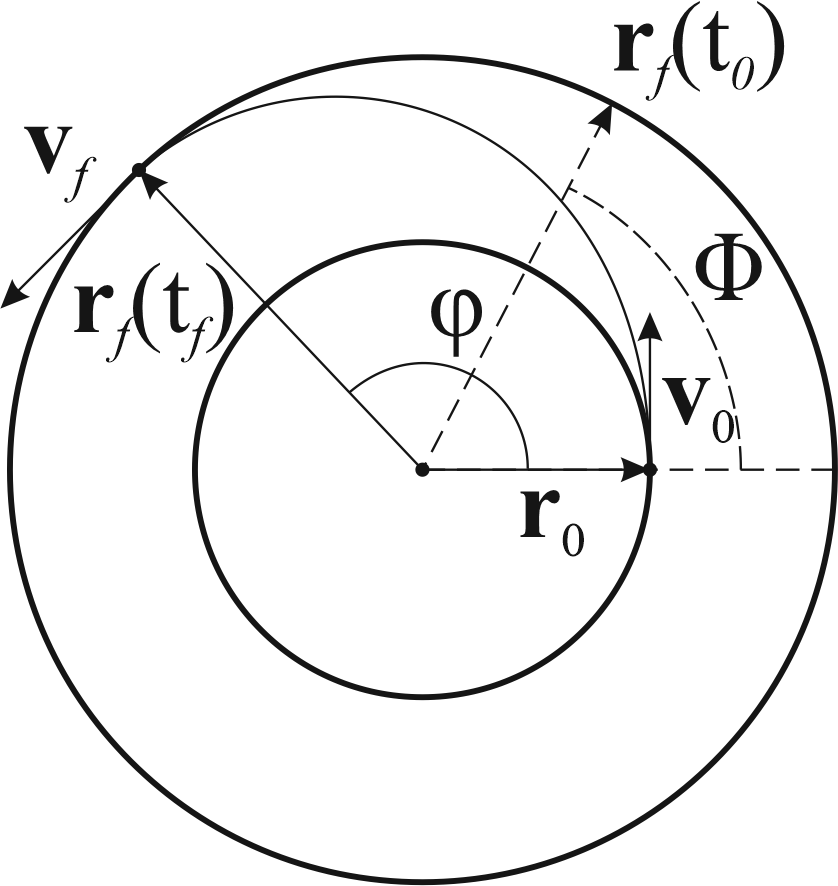
\includegraphics[width=0.37\textwidth]{virtual_planet.png}
    \caption{Модельная задача встречи виртуальных небесных тел на~круговых компланарных орбитах}
    \label{fig:syn-virtual-planets}
\end{figure}

Пусть $\boldsymbol\xi\in D_{\mathrm{reg}}\subset\mathbb R^h$ --- вектор $h$ внешних параметров задачи, $\mathbf z_0(\boldsymbol\xi)\in\mathbb R^6$ --- начальные значения сопряжённых переменных, а~$\mathbf c(\boldsymbol\xi)\in\mathbb R^n$ --- вектор $n$ характеристик траектории. Модельное многообразие определено как образ отображения, построенного на~одной регулярной связной ветви решений двухточечной краевой задачи энергетически оптимального перелёта:
\begin{equation}
    M:D_{\mathrm{reg}}\to\mathbb R^{6+n},\qquad
    M(\boldsymbol\xi)=\bigl(\mathbf z_0(\boldsymbol\xi),\mathbf c(\boldsymbol\xi)\bigr).
    \label{eq:syn-manifold}
\end{equation}
\par\noindent В~плоской круговой задаче используется двумерная сетка внешних параметров --- витковой дальности $\lambda=\varphi/(2\pi)$ и~отношения радиусов $\kappa$. Среди характеристик $\mathbf c$ рассматриваются продолжительность перелёта $T$, начальная синодическая фаза и~функционал $J$.

Многообразие строится дискретным продолжением по~координатной сетке: решение в~построенном узле служит начальным приближением в~соседнем.

После анализа геометрии, сечений и~областей регулярности многообразия его компоненты аппроксимируются непосредственно либо через иерархию коэффициент-функций. Формулы строятся методом символьной регрессии с~учётом точности, сложности и~согласованности, затем проверяются в~рабочей области повторным интегрированием расширенной системы.

\FloatBarrier
\Needspace*{6\baselineskip}
\noindent\textbf{Во второй главе} исследовано модельное многообразие в~плоской круговой модели, выделены кривая локальных оптимумов и~точки оптимальной дальности, а~их характеристики представлены конечными формулами. Исходная номограмма перелётов Земля--Марс в~координатах «дата старта --- продолжительность перелёта» расслаивается по~числу витков (рис.~\ref{fig:syn-start-date}), что затрудняет построение общей зависимости в~эфемеридной постановке.

\begin{figure}[htbp]
    \centering
    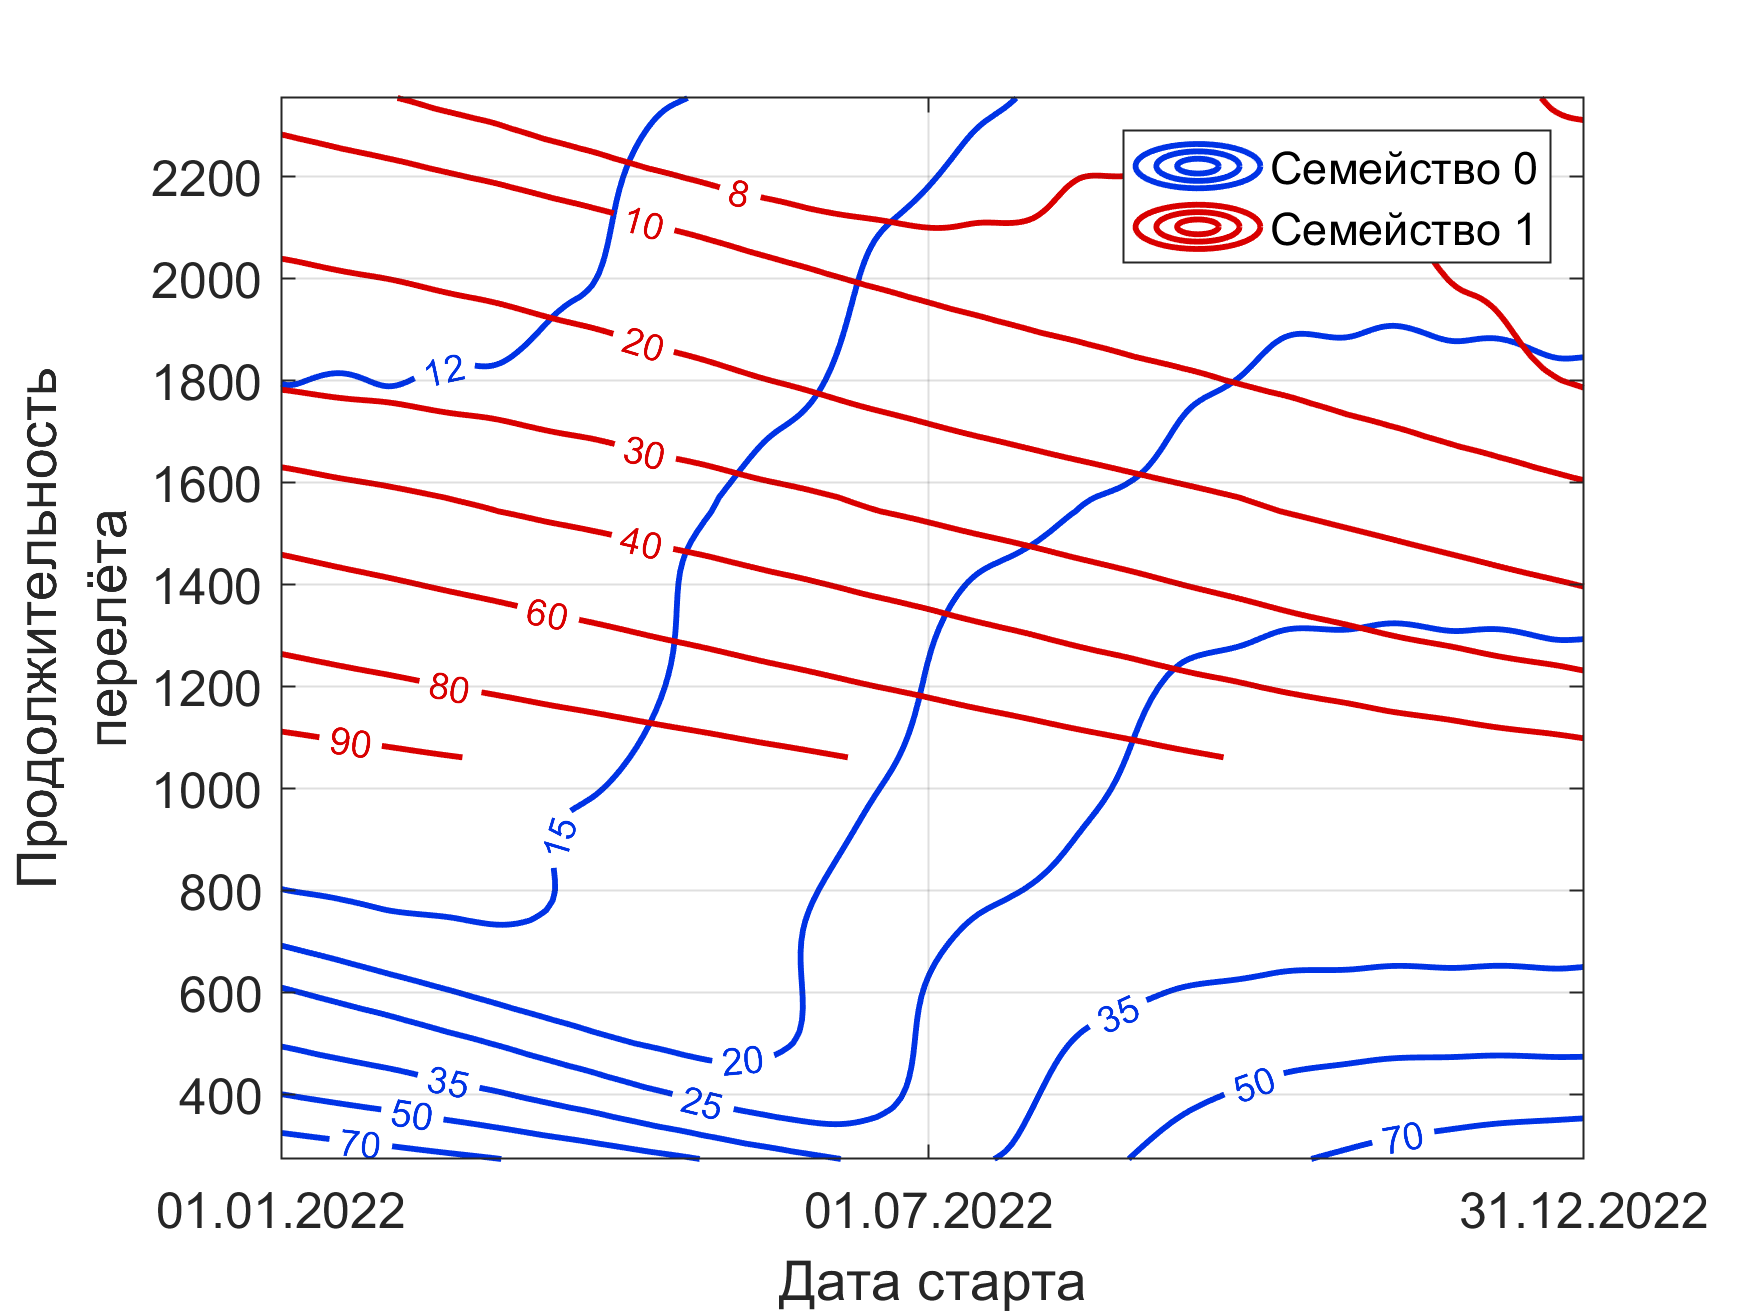
\includegraphics[width=0.82\textwidth]{StartDate_rebuilt2.png}
    \caption{Расслоение изолиний номограммы требуемого запаса рабочего тела для перелёта Земля--Марс}
    \label{fig:syn-start-date}
\end{figure}

В~модельной задаче вместо даты старта используется начальная синодическая фаза $\Phi$.

\noindent На~многообразии выделена \textit{кривая локальных оптимумов} (КЛО), состоящая из~решений, для которых при фиксированных $T$ и~$\kappa$ функционал имеет локальный минимум по~витковой дальности. Локально оптимальная витковая дальность обозначается $\lambda^\star$. КЛО строится как отдельная ветвь двухточечной задачи с~дополнительным условием на~свободный правый конец.

\looseness=-1 \textit{Точки оптимальной дальности} определены как счётное множество пересечений КЛО с~изолиниями фиксированной начальной синодической фазы (рис.~\ref{fig:syn-optimal-distance}). Одной фазе могут соответствовать несколько таких точек. Для устранения разрывов фазы на~границах периодов введена её нормированная непрерывная развёртка $\Psi$.

\begin{figure}[htbp]
    \centering
    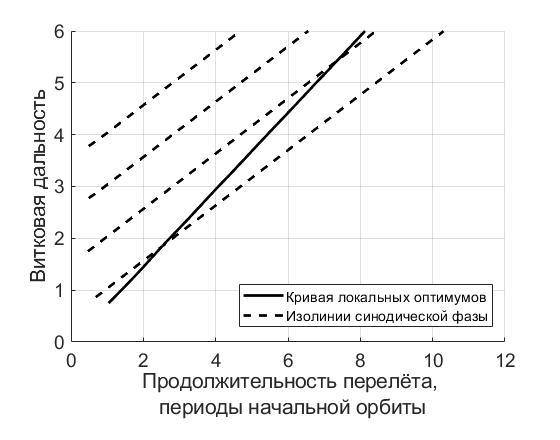
\includegraphics[width=0.76\textwidth]{Isolines.png}
    \caption{Точки оптимальной дальности как пересечения КЛО с~изолиниями начальной синодической фазы}
    \label{fig:syn-optimal-distance}
\end{figure}
\FloatBarrier

Для основной рабочей области $\lambda^\star\in[0.75,6]$, $\kappa\in[0.4,2.5]$ получены конечные формулы для $T$, $\Psi$, $J$ и~плоского вектора начальных значений сопряжённых переменных $\mathbf z_0^{\mathrm{pl}}$. Знаком $\widehat{\phantom{x}}$ далее обозначаются значения, вычисленные по~конечным формулам. Формула для продолжительности перелёта имеет вид
\begin{equation}
    \widehat T(\lambda^\star,\kappa)=
    \frac{2}{27}\kappa\ln\kappa
    +\lambda^\star\left(\kappa-\frac{\sqrt6}{9}\kappa\ln\kappa\right),
    \label{eq:syn-t-formula}
\end{equation}
причём $\widehat T(\lambda^\star,1)=\lambda^\star$, что согласуется с~предельным режимом совпадающих круговых орбит. Для восстановления зависимости $\widehat{\mathbf z}_0^{\mathrm{pl}}$ от~$\kappa$ использованы эталонные сечения $\kappa_1=0.72$ и~$\kappa_2=1.52$.
Хотя $\Psi=\lambda^\star-T/\kappa^{3/2}$, меньшую ошибку даёт самостоятельная конечная формула $\widehat\Psi=\mathcal A_0^{(\Psi)}(\kappa)+\mathcal A_1^{(\Psi)}(\kappa)\lambda^\star$, где коэффициент-функции $\mathcal A_0^{(\Psi)}$ и~$\mathcal A_1^{(\Psi)}$ зависят от~отношения радиусов $\kappa$.

Для даты старта с~нормированной фазой $\Psi_0=\Phi(t_0)/(2\pi)$ ветвь точек оптимальной дальности выбирается из~уравнений
\begin{equation}
    \widehat\Psi(\widehat\lambda_k^\star,\kappa)=\Psi_0+k,
    \qquad
    \widehat\lambda_k^\star=
    \frac{\Psi_0-\mathcal A_0^{(\Psi)}(\kappa)+k}
         {\mathcal A_1^{(\Psi)}(\kappa)},
    \quad k\in\mathbb Z.
\end{equation}
Затем по~формуле~\eqref{eq:syn-t-formula} вычисляется $\widehat T_k$, $\widehat J$ служит оценкой энергетического функционала, а~$\widehat{\mathbf z}_0^{\mathrm{pl}}$ --- начальным приближением краевой задачи. Для сопряжённых переменных выявлена попарная структура $(p_{rx},p_{vy})$ и~$(p_{ry},p_{vx})$.

В~табл.~\ref{tab:syn-main-errors} приведены ошибки безразмерных конечных формул: среднеквадратическая (RMSE), средняя абсолютная (MAE) и~максимальная абсолютная; $S$ --- характерный масштаб величины.

\begin{table}[htbp]
    \centering
    \caption{Ошибки конечных формул в~основной рабочей области}
    \label{tab:syn-main-errors}
    \small
    \begin{tabular}{@{}lcccc@{}}
        \toprule
        Величина & $S$ & RMSE & MAE & $\max|\Delta|$ \\
        \midrule
        $\widehat T$ & $4.96\!\times\!10^{0}$ & $2.32\!\times\!10^{-2}$ & $1.46\!\times\!10^{-2}$ & $1.44\!\times\!10^{-1}$ \\
        $\widehat\Psi$ & $1.41\!\times\!10^{0}$ & $1.88\!\times\!10^{-2}$ & $1.27\!\times\!10^{-2}$ & $1.04\!\times\!10^{-1}$ \\
        $\widehat J$ & $5.28\!\times\!10^{-3}$ & $1.24\!\times\!10^{-4}$ & $3.39\!\times\!10^{-5}$ & $2.69\!\times\!10^{-3}$ \\
        $\widehat{\mathbf z}_0^{\mathrm{pl}}$ & $3.22\!\times\!10^{-2}$ & $8.71\!\times\!10^{-4}$ & $1.75\!\times\!10^{-4}$ & $3.36\!\times\!10^{-2}$ \\
        \bottomrule
    \end{tabular}
\end{table}

\FloatBarrier
\noindent\textbf{В третьей главе} разработаны три типа линейных $R$-преобразований сопряжённых переменных для перехода от~плоской круговой модели к~постановкам с~изменённым начальным фазовым вектором, эллиптической и~пространственной конечной орбитой. Их композиция преобразует модельный сопряжённый вектор для целевой задачи встречи.

Общей конструкцией служит матричная функция $R$ двух векторных аргументов. Паре неколлинеарных векторов $\boldsymbol\rho,\boldsymbol\nu\in\mathbb R^3$ она сопоставляет матрицу
\begin{equation}
    R(\boldsymbol\rho,\boldsymbol\nu)=
    \begin{pmatrix}\boldsymbol\rho&\boldsymbol\nu&\boldsymbol\rho\times\boldsymbol\nu\end{pmatrix}.
    \label{eq:syn-r-general}
\end{equation}
При заданных аргументах $R(\boldsymbol\rho,\boldsymbol\nu)$ --- конкретная невырожденная матрица; далее, когда аргументы ясны из~контекста, она обозначается $R$. С~выбранной матрицей связаны правила преобразования вектора $\mathbf y'=R\mathbf y$ и~сопряжённого ковектора $\mathbf p'=(R^{\mathsf T})^{-1}\mathbf p$.

Выбор аргументов функции и~способ применения полученной матрицы зависят от~типа преобразования. В~I типе изменяются начальные фазовый и~сопряжённый векторы; во~II и~III типах преобразуются только начальные значения сопряжённых переменных. Структура матриц II и~III типов выбирается с~учётом изменения значений первых интегралов расширенной системы, включая $\mathbf M=\mathbf r\times\mathbf p_r+\mathbf v\times\mathbf p_v$. После преобразования начальных данных расширенная система интегрируется заново.

\noindent\textit{$R$-преобразование I~типа.} Преобразование применяется при изменении начального фазового вектора. Для пар $\mathbf x_a=(\mathbf r_a,\mathbf v_a)$ и~$\mathbf x_b=(\mathbf r_b,\mathbf v_b)$ матрица перехода имеет вид
\begin{equation}
    R_{a\to b}=R_bR_a^{-1},
    \qquad
    \mathbf p_{r,b}=R_{a\to b}^{-\mathsf T}\mathbf p_{r,a},
    \qquad
    \mathbf p_{v,b}=R_{a\to b}^{-\mathsf T}\mathbf p_{v,a}.
    \label{eq:syn-r-type1}
\end{equation}
Здесь $R_a=R(\mathbf r_a,\mathbf v_a)$ и~$R_b=R(\mathbf r_b,\mathbf v_b)$ построены для исходного и~целевого фазовых векторов. В~отличие от~простого поворота преобразование учитывает масштаб и~взаимное расположение начальных векторов положения и~скорости и~даёт меньшие невязки правого конца.

\Needspace*{8\baselineskip}
\noindent\textit{$R$-преобразование II~типа.} При фиксированных $\mathbf r_0$, $\mathbf v_0$ оно задаёт эксцентриситет $e$ и~аргумент перицентра $\omega$ конечной орбиты. Параметр $\zeta$ деформирует матрицу $R_e$, ориентированную поворотом $Q_\chi$ вокруг оси $Oz$: $R_{e\omega}=Q_\chi R_eQ_\chi^{\mathsf T}$.
Угол поворота $\chi$ и~управляющий параметр $\zeta$ вычисляются по~конечным формулам
\begin{equation}
\begin{gathered}
    \chi(\omega)=\frac{\omega}{2}+\frac16\sin2\omega+\frac1{32}\sin4\omega,\\
    \zeta=-\frac{e}{\mathcal A^{(e)}(\kappa,\omega)},
\end{gathered}
\label{eq:syn-r-type2-control}
\end{equation}
где $\mathcal A^{(e)}$ --- коэффициент-функция чувствительности с~гармонической структурой по~$\omega$. Побочное изменение витковой дальности компенсируется сдвигом точки модельного многообразия:
\begin{equation}
    \lambda_{\mathrm{corr}}=
    \lambda-\frac{1}{2\pi}\mathcal B_\lambda(\omega,\lambda,\kappa)\zeta.
    \label{eq:syn-lambda-correction}
\end{equation}
Здесь $\mathcal B_\lambda$ --- локальная чувствительность полного угла к~$\zeta$. Коррекция уменьшила RMSE витковой дальности с~$7.31\times10^{-2}$ до~$1.66\times10^{-2}$.

\noindent\textit{$R$-преобразование III~типа.} Преобразование предназначено для задания наклонения $i$ и~долготы восходящего узла $\Omega$. При фиксированном начальном фазовом векторе используется базовая матрица $R_i(j)$, параметризованная управляющей величиной $j$, а~её ориентация задаётся матрицей $Q_\Omega$ поворота вокруг оси $Oz$ на~угол $\Omega$:
\begin{equation}
    R_i(j)=
    \begin{pmatrix}
        1&0&0\\
        0&(1+j^2)^{-1}&-j(1+j^2)^{-1}\\
        0&j(1+j^2)^{-1}&(1+j^2)^{-1}
    \end{pmatrix},
    \qquad
    R_{i\Omega}=Q_\Omega R_iQ_\Omega^{\mathsf T},
\end{equation}
а~управляющий параметр определяется формулой $j=-i/\mathcal A^{(i)}(\kappa,\Omega)$.\par\noindent
Коэффициент-функция $\mathcal A^{(i)}=\mathcal A_0^{(i)}(\kappa)+\mathcal A_1^{(i)}(\kappa)\cos2\Omega$ задаёт локальную чувствительность наклонения к~$j$. RMSE задания $i$ и~$\Omega$ составили $3.01\times10^{-3}$ и~$1.12\times10^{-2}$~рад, максимальные ошибки --- $1.22\times10^{-2}$ и~$3.36\times10^{-2}$~рад. Из-за побочных изменений $\lambda$ и~большой полуоси $a$ результат преобразования используется как начальное приближение с~последующим уточнением.

Для учёта полной геометрии задачи преобразования объединяются в~композицию. По~$\lambda_{\mathrm{corr}}$ и~$\kappa$ вычисляются модельные сопряжённые векторы, $R_0$ согласует модельный и~реальный начальные фазовые векторы, затем учитываются эллиптичность и~пространственная ориентация:
\begin{equation}
\begin{gathered}
    R_\Sigma=R_{i\Omega}(j,\gamma)
              R_{e\omega}(\zeta,\bar\omega_{\mathrm{rel}})R_0,\\
    \mathbf p_{r0}^{\mathrm{init}}=R_\Sigma^{-\mathsf T}
       \widehat{\mathbf p}_{r0}^{\mathrm{corr}},
    \qquad
    \mathbf p_{v0}^{\mathrm{init}}=R_\Sigma^{-\mathsf T}
       \widehat{\mathbf p}_{v0}^{\mathrm{corr}},
\end{gathered}
\label{eq:syn-r-composition}
\end{equation}
где $\bar\omega_{\mathrm{rel}}=\Omega+\omega-L_0$, $\gamma=\Omega-L_0$, $L_0$ --- истинная долгота начального радиус-вектора. Композиция формирует геометрически согласованное начальное приближение для численной коррекции. Последовательное применение трёх типов преобразований показано на~рис.~\ref{fig:syn-r-composition}.

\begin{figure}[htbp]
    \centering
    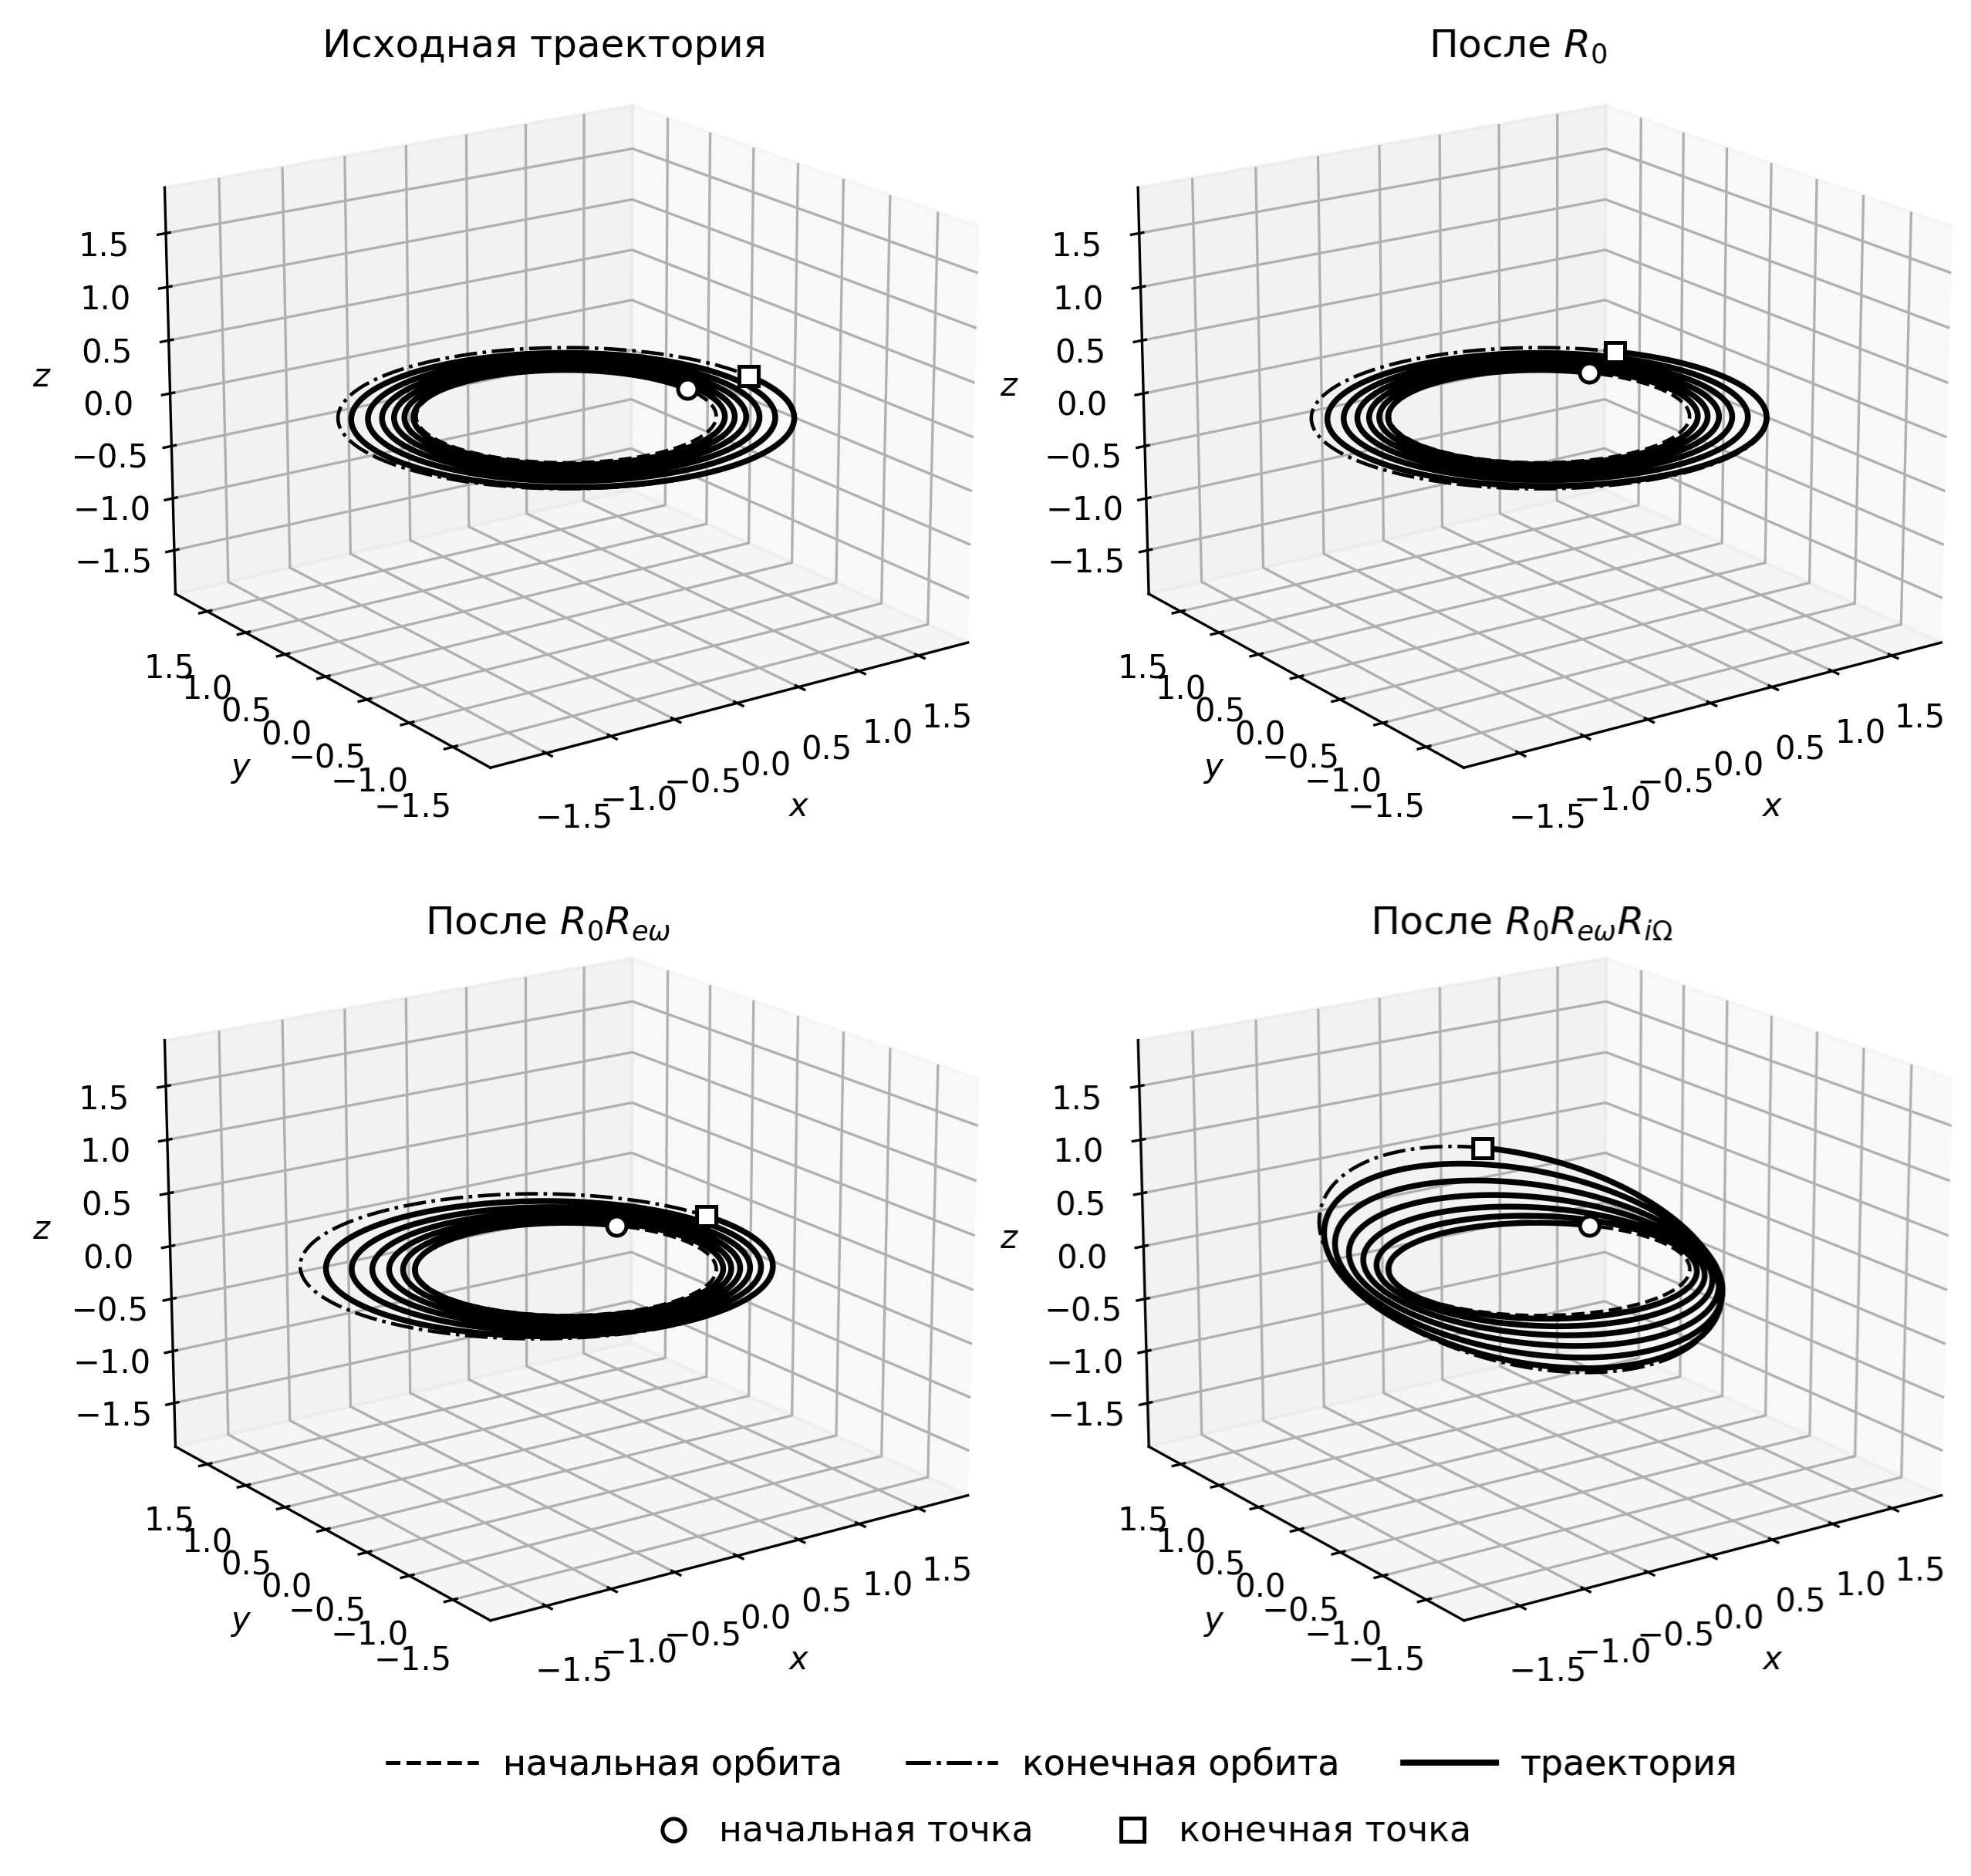
\includegraphics[width=0.70\textwidth]{R_composition_sequential_example.png}
    \caption{Изменение исходной траектории при последовательном применении $R$-преобразований I, II и~III~типов}
    \label{fig:syn-r-composition}
\end{figure}

\FloatBarrier
\noindent\textbf{В четвёртой главе} конечные формулы и~$R$-преобразования объединены в~алгоритм построения начального приближения по~дате старта и~целевым орбитальным параметрам. Управляющий вектор $\mathbf q=(\lambda,\kappa,\zeta,\chi,j,\gamma)$ имеет геометрический смысл: пара $(\lambda,\kappa)$ задаёт точку модельного многообразия, $\zeta$ и~$\chi$ задают эксцентриситет и~линию апсид, $j$ и~$\gamma$ --- наклонение и~линию узлов. Это заменяет прямой подбор шести сопряжённых переменных.

Алгоритм состоит из~следующих шагов:
\begin{enumerate}
    \item по~эфемеридам для заданной даты старта определяются начальный фазовый вектор и~элементы целевой орбиты, после чего выполняется переход к~безразмерной постановке;
    \item по~начальной синодической фазе находятся три ближайшие точки оптимальной дальности $\lambda_k^\star$, $k\in\{-1,0,1\}$;
    \item исключаются кандидаты вне физически допустимой области $T>0$ и~области применимости формул, из~оставшихся выбирается вариант, удовлетворяющий ограничениям и~дающий лучшее значение критерия;
    \item точка КЛО корректируется по~формуле~\eqref{eq:syn-lambda-correction}, затем вычисляются $\widehat T$, $\widehat J$ и~$\widehat{\mathbf z}_0^{\mathrm{pl}}$;
    \item композиция~\eqref{eq:syn-r-composition} переводит модельное решение в~начальный вектор расширенной системы $\mathbf y_0^{\mathrm{init}}$ эфемеридной задачи;
    \item $\mathbf y_0^{\mathrm{init}}$ и~$\widehat T$ используются для последующего численного решения двухточечной краевой задачи.
\end{enumerate}

Для перелёта Земля--Марс по~эфемеридам JPL DE430 получены $\lambda^\star=1.324$, $\lambda_{\mathrm{corr}}=1.269$ и~$\kappa=1.524$. Табл.~\ref{tab:syn-mars-refinement} показывает попадание начального приближения в~область сходимости и~результат уточнения.

\begin{table}[htbp]
    \centering
    \caption{Уточнение начального приближения для перелёта Земля--Марс}
    \label{tab:syn-mars-refinement}
    \small
    \begin{tabular}{@{}lcc@{}}
        \toprule
        Величина & Начальное приближение & После уточнения \\
        \midrule
        Продолжительность, сут. & $636.2$ & $653.8$ \\
        Норма невязки положения, км & $6.54\times10^{7}$ & $8.07\times10^{-4}$ \\
        Норма невязки скорости, км/с & $8.88$ & $9.41\times10^{-11}$ \\
        \bottomrule
    \end{tabular}
\end{table}

Сравнение начального приближения и~уточнённой траектории показано на~рис.~\ref{fig:syn-mars-initial-refined}.

\begin{figure}[htbp]
    \centering
    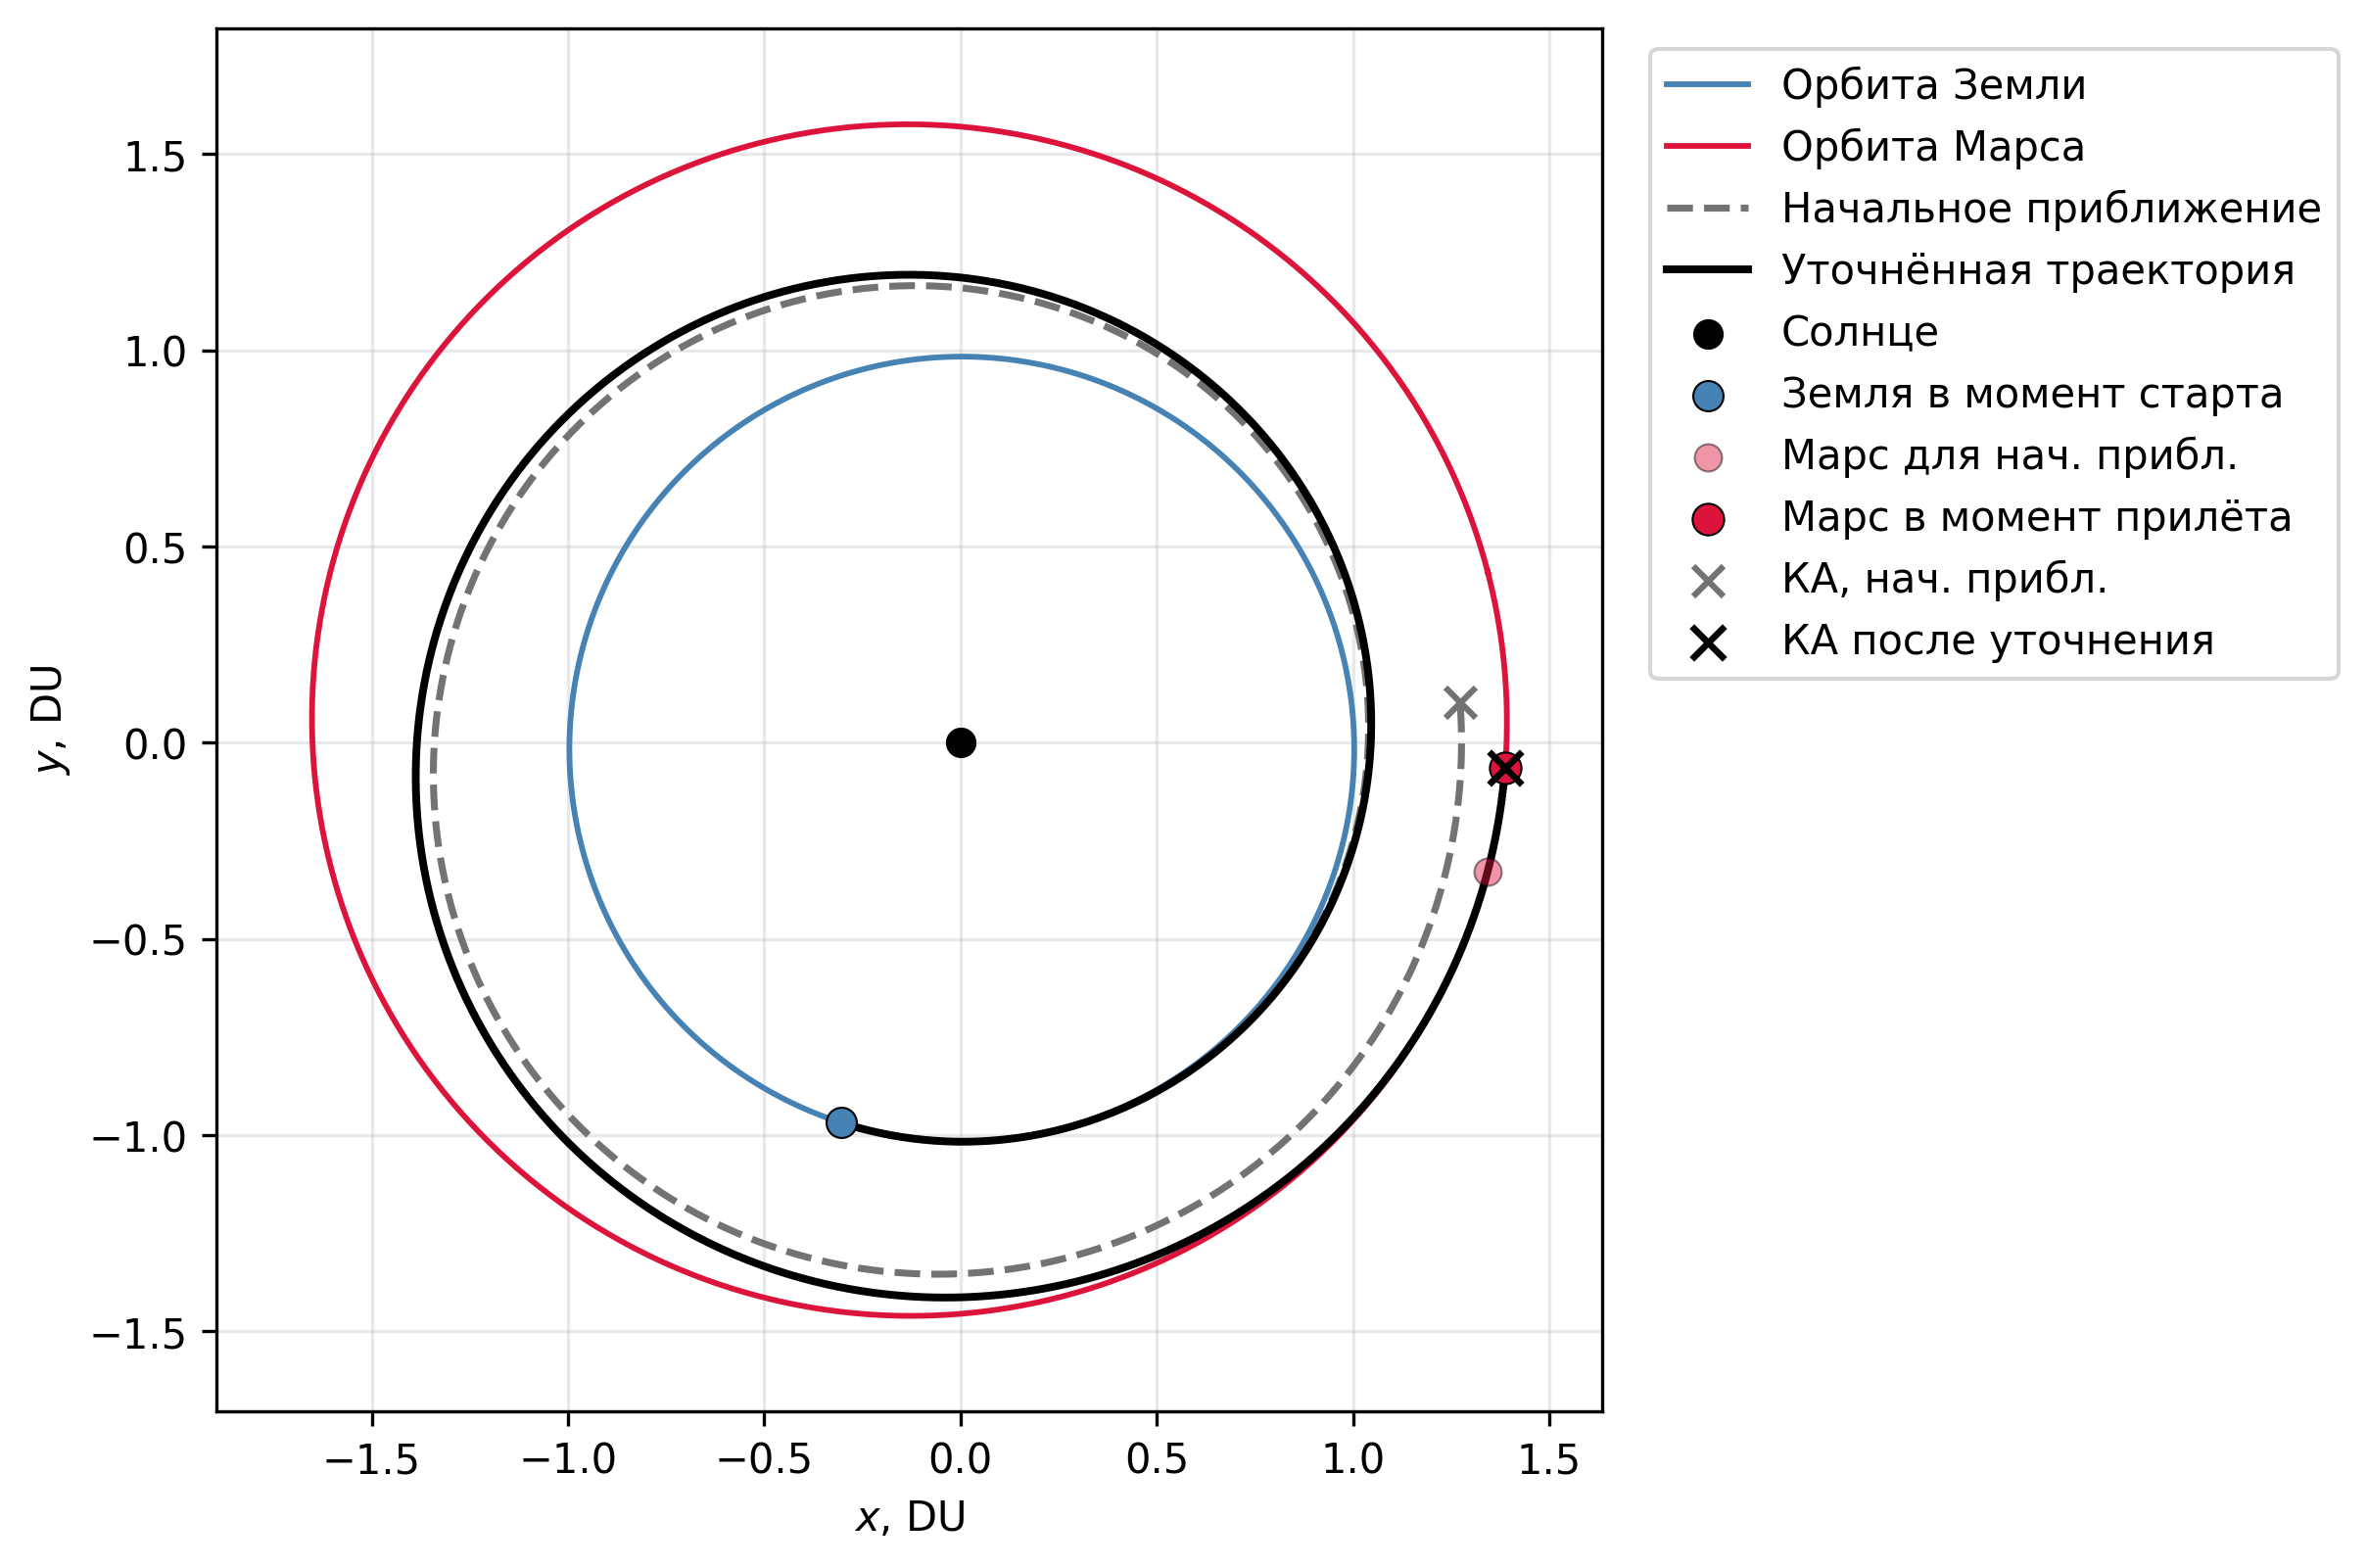
\includegraphics[width=0.80\textwidth]{chap4_mars_cleanver_rebuilt_Oxy.png}
    \caption{Сравнение начального приближения и~уточнённой траектории для перелёта Земля--Марс}
    \label{fig:syn-mars-initial-refined}
\end{figure}

Устойчивость проверена на~эфемеридных конфигурациях, охватывающих 17-летний цикл Земли и~Марса и~8-летний цикл Земли и~Венеры. В~табл.~\ref{tab:syn-mission-quality} приведены средние по~всем датам абсолютные ошибки до~уточнения; оптимизация в~параметрах $\mathbf q$ снижала невязки элементов конечной орбиты до~$10^{-12}$--$10^{-15}$.

\begin{table}[htbp]
    \centering
    \caption{Средние абсолютные ошибки начального приближения}
    \label{tab:syn-mission-quality}
    \small
    \renewcommand{\arraystretch}{0.9}
    \begin{tabular}{lcc}
        \toprule
        Параметр & Земля--Марс & Земля--Венера \\
        \midrule
        $e$ & $3.0\times10^{-3}$ & $2.0\times10^{-2}$ \\
        $i$, град & $4.0\times10^{-3}$ & $2.0\times10^{-1}$ \\
        $\Omega$, град & $4.0$ & $2.0$ \\
        $\omega$, град & $11$ & $26$ \\
        $\varphi$, град & $3.0$ & $0.7$ \\
        $a$, а.е. & $6.0\times10^{-2}$ & $4.0\times10^{-3}$ \\
        $J$, м$^2$/с$^3$ & $8.0\times10^{-2}$ & $3.0\times10^{-3}$ \\
        $T$, сут. & $8.5$ & $0.7$ \\
        \bottomrule
    \end{tabular}
\end{table}

Сравнение с~продолжением по~гравитационному параметру $\mu$ выполнено на~одном процессоре с~использованием Python для 100 дат старта к~Марсу с~шагом 15~суток, начиная с~1~января 2026~г. (табл.~\ref{tab:syn-method-comparison}).

\begin{table}[htbp]
    \centering
    \caption{Сравнение способов формирования и~уточнения начального приближения}
    \label{tab:syn-method-comparison}
    \small
    \begin{tabular}{@{}lcccc@{}}
        \toprule
        Метод & Решено задач & Время, с & Интегрирований & Проверено ветвей \\
        \midrule
        Предлагаемый подход & 100 из 100 & $0.636$ & $70.3$ & --- \\
        Продолжение по~$\mu$ & 100 из 100 & $1.89$ & $43.0$ & $3.8$ \\
        \bottomrule
    \end{tabular}
\end{table}

\FloatBarrier
Оба способа обеспечили машинную точность во~всех задачах. Продолжение по~$\mu$ запускалось для нескольких номеров ветви с~последующим выбором лучшего решения. Предлагаемый метод не~требует заранее задавать номер ветви.

Полученное ИРТ-решение используется как исходная точка для двух последовательных продолжений к~более прикладной постановке. Первое продолжение вводит дополнительный импульс скорости. При параметре $\tau_1\in[0,1]$ начальная скорость задаётся как
\begin{equation}
    \mathbf v(t_0)=\mathbf v_C(t_0)
    +\tau_1v_{\delta,\max}\mathbf n_\delta(\tau_1),
    \qquad
    \mathbf n_\delta(\tau_1)=
    \frac{\mathbf p_{v0}(\tau_1)}{\lVert\mathbf p_{v0}(\tau_1)\rVert}.
    \label{eq:syn-vdelta-continuation}
\end{equation}
Здесь $\mathbf v_C(t_0)$ --- скорость тела отправления, $v_{\delta,\max}$ --- заданный предельный модуль дополнительного импульса. При $\tau_1=0$ дополнительный импульс отсутствует; при $\tau_1=1$ достигается его предельное значение. Направление выбирается согласованно с~условием трансверсальности, а~конечные формулы и~$R$-преобразования задают начальное решение для $\tau_1=0$.

Второе продолжение переводит полученное ИРТ-решение с~дополнительным импульсом к~модели постоянной скорости истечения. Квадратичный функционал деформируется в~линейный по~модулю реактивного ускорения:
\begin{equation}
    J_{\tau_2}=\int_{t_0}^{t_0+T}
    \left((1-\tau_2)\frac{\lVert\mathbf a(t)\rVert^2}{2}
    +\tau_2\lVert\mathbf a(t)\rVert\right)dt,
    \qquad \tau_2\in[0,1].
    \label{eq:syn-psi-continuation}
\end{equation}
Значения $\tau_2=0$ и~$\tau_2=1$ соответствуют ИРТ- и~ПСИ-постановкам. Для обоих продолжений изменение начального вектора $\mathbf z_0$ определяется из~системы невязок $\mathbf F(\mathbf z_0,\tau_\ell)=\mathbf0$:
\begin{equation}
    \frac{d\mathbf z_0}{d\tau_\ell}=
    -\left(\frac{\partial\mathbf F}{\partial\mathbf z_0}\right)^{-1}
    \frac{\partial\mathbf F}{\partial\tau_\ell},
    \qquad \ell=1,2.
    \label{eq:syn-two-continuations}
\end{equation}
Для перелёта Земля--Венера при начальной массе 156~кг получено опорное ПСИ-решение продолжительностью 390.8~суток с~моторным временем 195.2~суток, затратами топлива 41.77~кг и~дополнительным импульсом 2.67~км/с.

Конечные формулы, $R$-преобразования, интегрирование расширенной системы и~уточнение в~параметрах $\mathbf q$ реализованы в~комплексе \texttt{ILTT Toolbox}.

\FloatBarrier
\pdfbookmark[1]{Основные результаты и выводы}{main-results}
\section*{Основные результаты и выводы}

\begin{enumerate}
    \item Построено регулярное модельное многообразие энергетически оптимальных решений задачи встречи с~идеально регулируемой тягой. Показано, что расслоение многовитковых решений переходит в~односвязное многообразие, на~котором выделены кривая локальных оптимумов и~точки оптимальной дальности.

    \item В~области $\lambda^\star\in[0.75,6]$, $\kappa\in[0.4,2.5]$ получены конечные формулы для продолжительности перелёта, непрерывной фазы, функционала и~начальных значений сопряжённых переменных. RMSE составила $2.32\times10^{-2}$ для $\widehat T$, $1.88\times10^{-2}$ для $\widehat\Psi$, $1.24\times10^{-4}$ для $\widehat J$ и~$8.71\times10^{-4}$ для $\widehat{\mathbf z}_0^{\mathrm{pl}}$.

    \item Разработаны три типа линейных $R$-преобразований: для изменения начального фазового вектора, задания эксцентриситета и~линии апсид, наклонения и~линии узлов конечной орбиты. Установлены побочные изменения, вызываемые этими преобразованиями, и~вырожденные случаи; коррекция уменьшила RMSE витковой дальности с~$7.31\times10^{-2}$ до~$1.66\times10^{-2}$.

    \item Предложен алгоритм, который по~дате старта проверяет не~более трёх точек оптимальной дальности и~преобразует модельный сопряжённый вектор для целевой задачи. На~сетке из~100 дат старта перелёта к~Марсу получено 100\% успешных уточнений при среднем времени $0.636$~с против $1.89$~с для продолжения по~$\mu$. ИРТ-решение последовательно продолжено по~дополнительному импульсу скорости и~к~ПСИ-постановке; для перелёта Земля--Венера получено опорное решение с~затратами топлива 41.77~кг и~дополнительным импульсом 2.67~км/с. Схема реализована в~\texttt{ILTT Toolbox}.
\end{enumerate}

\renewcommand{\bibtitleauthor}{Список публикаций по теме диссертации}
\nocite{%
korneev_low_thrust_ks_2024,
korneev_parametric_analysis_2025,
korneev_regular_variables_2022,
korneev_mars_platform_2024,
korneev_venus_platform_2026,
korneev_affine_transformations_2025,
korneev_symbolic_regression_2024,
korneev_duration_ngpm_2024,
korneev_hybrid_mars_2024,
korneev_exhaustive_parametric_2024,
korneev_coplanar_circular_2025,
korneev_affine_noncoplanar_2025,
korneev_elliptic_circular_2025,
korneev_solution_structure_mipt_2023,
korneev_ks_canonical_2022,
korneev_phase_variables_2021,
korneev_regularized_trajectory_2020,
korneev_propulsion_2024,
korneev_fakel_2025,
prog_iltt_toolbox}
\begingroup
\small
\setlength{\bibhang}{1em}
\setlength{\bibitemsep}{0pt}
\Urlmuskip=0mu
\urlstyle{same}
\section*{\bibtitleauthor}
\printbibliography[heading=pubsubgroup,section=0,keyword=biblioauthorvak,
    title={Публикации в~изданиях, рекомендованных ВАК},resetnumbers=true]
\defbibfilter{synopsisother}{%
    keyword=biblioauthorconf or keyword=biblioauthorother
}
\printbibliography[heading=pubsubgroup,section=0,filter=synopsisother,
    title={Другие научные публикации по~теме диссертации},resetnumbers=false]
\printbibliography[heading=pubsubgroup,section=0,keyword=biblioauthorprogram,
    title={Свидетельство о~государственной регистрации программы для ЭВМ},resetnumbers=false]
\endgroup
      % Содержание автореферата

%%% Выходные сведения типографии
\par\vfill
\begingroup
\footnotesize
\noindent
{\centering
Подписано в~печать \blank[\widthof{00}].\blank[\widthof{00}].2026.
Формат 60\(\times\)84/16. Усл. печ. л. 1,2. Тираж 70~экз. Заказ \blank[\widthof{А-ххх}].

ИПМ им.~М.В.~Келдыша РАН. 125047, Москва, Миусская пл., 4
\par}
\endgroup
\end{document}
